View demo code of this section: \demonotebook{05}{5.4.2}

\subsubsection{Background}
Variational quantum algorithms have been primarily focused on identifying the ground state of complex many-body systems. In this context, the Variational Quantum Eigensolver (VQE) algorithm, designed to find the ground state of a many-body system  by minimizing its average energy, has emerged as a powerful tool. However, several critical phenomena in physics, including topological phases, necessitate knowledge of several low-energy eigenstates, not just the ground state. Consequently, extending VQE to higher energy eigenstates is of significant importance.

The weighted SSVQE method offers an alternative approach to generate all the $k$ lowest energy eigenstates of a given Hamiltonian $H$~\cite{nakanishi2019subspace}. This method utilizes a set of $k$ orthogonal initial states, denoted as $\{|\phi_{i}\rangle\}_{i=1}^{k}$ (where $\langle \phi_{i} | \phi_{j} \rangle = \delta_{ij}$), as inputs for a single parameterized quantum circuit, described by the unitary operator $U(\vec{\theta})$. Given that the initial states are orthogonal, the outputs $U(\vec{\theta})| \phi_{j} \rangle$, generated by the same circuit, maintain orthogonality. In the weighted SSVQE, the objective is to minimize the cost function
\begin{equation}
    \mathrm{cost} = \sum_{i=1}^{k} w_{i} \langle \phi_{i}| U^{\dagger}(\vec{\theta}) H U(\vec{\theta}) | \phi_{i} \rangle
    \label{ssvqe_cost}
\end{equation}
where $w_1 > w_2 > \cdots > w_k$ are real positive numbers. Minimizing the cost function in Eq.~\eqref{ssvqe_cost} produces all the $k$ lowest energy eigenstates such that $|E_{i}\rangle = U(\vec{\theta}^{*})|\phi_{i}\rangle$.
A notable advantage of the weighted SSVQE is that it delivers all the $k$ lowest energy eigenstates through a single optimization process, without requiring any evaluation of quantum state overlaps. However, the algorithm becomes more resource-demanding as the number of target eigenstates increases.

Symmetry stands as one of the most fundamental concepts in physics, particularly in quantum mechanics. A majority of physical systems exhibit various types of symmetries that can be accurately described mathematically. The VQE algorithm can also significantly benefit from the integration of these symmetries. There are two ways to incorporate symmetries in the VQE algorithms: (i) designing the circuit to naturally generate the quantum states with the relevant symmetry~\cite{Lyu2020accelerated,Gard2020,barron2021preserving}, and (ii) adding extra terms to the cost function to penalize the quantum states without the relevant symmetry~\cite{mcclean2016theory,ryabinkin2018constrained}.

\subsubsection{Implementation}
Using the adaptable and comprehensive features of \MindQuantum, researchers can address various optimization targets by defining custom objective functions. In this section, we demonstrate the implementation of SSVQE using \MindQuantum to precisely determine the four lowest state energies of the Heisenberg Hamiltonian, while incorporating various symmetry strategies.

Initially, the construction of a symmetry-preserving ansatz is necessary, as detailed in Ref.~\cite{Lyu2023symmetryenhanced}.
\begin{lstlisting}
def entangling_gate(parameter, qubits):
    circuit = Circuit()
    circuit += RZ(-np.pi / 2).on(qubits[1])
    circuit += CNOT.on(qubits[0], qubits[1])
    circuit += RZ({parameter: -2}).on(qubits[0])
    circuit += RZ(np.pi / 2).on(qubits[0])
    circuit += RY({parameter: 2}).on(qubits[1])
    circuit += RY(-np.pi / 2).on(qubits[1])
    circuit += CNOT.on(qubits[1], qubits[0])
    circuit += RY({parameter: -2}).on(qubits[1])
    circuit += RY(np.pi / 2).on(qubits[1])
    circuit += CNOT.on(qubits[0], qubits[1])
    circuit += RZ(np.pi / 2).on(qubits[0])
    return circuit

def ansatz(N, layers, local_rot=True):
    circuit = Circuit()
    params_index = 0
    for layer_index in range(layers):
        for i in range(2):
            for j in range(i, N - 1, 2):
                circuit += entangling_gate(str(params_index), [j, j + 1])
                params_index += 1
        if local_rot:
            for i in range(N):
                circuit += PhaseShift(params_index).on(i)
                params_index += 1
    return circuit
\end{lstlisting}

SSVQE can be implemented as a combination of several VQEs, each with distinct initialization circuits but sharing a common parameterized ansatz.
For most VQE instance, specific tasks are defined by their corresponding measurement functions.
Using the \getexpectationwithgrad function, one can easily obtain the expectation value and the corresponding gradient with respect to the trainable variables. Here, as an example, we demonstrate the code implementation for obtaining the second- and the third-lowest state energies of the Heisenberg Hamiltonian. In this particular instance,
we use a $S_z$-conserving ansatz, which preserves the $z$ component of the total spin, and the total spin operator is added to the cost function as a penalty term. The cost function is then modified into a form of
\begin{equation}
    \mathrm{cost} = \sum_{i=1}^{k} w_{i} \langle \phi_{i}| U^{\dagger}(\vec{\theta}) [H + \beta(\hat{O} - c)^2] U(\vec{\theta}) | \phi_{i} \rangle,
    \label{ssvqe_cost_pen}
\end{equation}
where $c$ is a constant indicating the target subspace, and $\beta$ is a positive constant which is taken to be sufficiently large according to the form of penalty terms. Here, we do the expansion $(\hat{O} - c)^2 {=} \hat{O}^2 {-} c\hat{O} {+} c^2$. Together with the Hamiltonian, now we have three different measurement operators. The corresponding measurement operators in the case of Heisenberg Hamiltonian and the total spin operator can be generated with the following codes.

\begin{lstlisting}
def s_alpha(N, alpha: str = 'X'):
    alpha = alpha.upper()
    out = QubitOperator()
    for i in range(N):
        out += QubitOperator(alpha + f'{i}')
    return out * 0.5

def s_tot_op(N):
    s_x_op = s_alpha(N, 'X')**2
    s_y_op = s_alpha(N, 'Y')**2
    s_z_op = s_alpha(N, 'Z')**2
    op = s_x_op + s_y_op + s_z_op
    op.compress()
    return op

def ham_heis(n_qubits, J):
    ham = QubitOperator()
    for i in range(1, n_qubits):
        ham += QubitOperator("X{} X{}".format(i - 1, i), J)
        ham += QubitOperator("Y{} Y{}".format(i - 1, i), J)
        ham += QubitOperator("Z{} Z{}".format(i - 1, i), J)
    ham.compress()
    return Hamiltonian(ham)
\end{lstlisting}

Having predefined all necessary modules, including the initialization circuits, shared parameter ansatz, measurement operators, and the constant $\beta$, we can proceed with implementing the SSVQE algorithm. The following code snippet shows the implementation of the SSVQE class.
\begin{lstlisting}
class SSVQE:
    def __init__(self, n_qubits, init_circuits, pqc, ops, beta):
        self.n_qubits = n_qubits
        self.circs = [circ + pqc for circ in init_circuits]
        self.sim = Simulator('mqvector', n_qubits)
        self.beta = beta
        self.grad_ops = [self.sim.get_expectation_with_grad(ops, circ) for circ in self.circs]

    def energy(self, params):
        if self.sim is None:
            self.sim = Simulator('mqvector', self.n_qubits)
        energies = []
        for i in range(len(self.grad_ops)):
            f, g = self.grad_ops[i](params)
            energies.append(f[0, 0].real)
        return energies

    def __call__(self, inputs):
        cost = 0
        cost_grad = 0
        for i in range(len(self.grad_ops)):
            f, g = self.grad_ops[i](inputs)
            f1, f2, f3 = f[0, 0].real, f[0, 1].real, f[0, 2].real
            g1, g2, g3 = np.array(g[0, 0, :].real), np.array(g[0, 1, :].real), np.array(g[0, 2, :].real)
            cost += (f1 + self.beta * (f2 + f3)) * (len(self.grad_ops) - i)
            cost_grad += (g1 + self.beta * (g2 + g3)) * (len(self.grad_ops) - i)
        return cost, cost_grad
\end{lstlisting}


Upon completion of the algorithm implementation, the focus shifts to SSVQE optimization. The choice of classical optimizer remains flexible. For this instance, the "L-BFGS-B" optimizer from SciPy is selected.


\begin{lstlisting}
initial_parameter = (np.random.rand(len(ssvqe.circs[0].params_name)) - .5) * np.pi
res = scipy.optimize.minimize(ssvqe,
                    initial_parameter,
                    method='l-bfgs-b',
                    jac=True,
                    options={'disp': False})
\end{lstlisting}

\begin{figure}
	\centering
	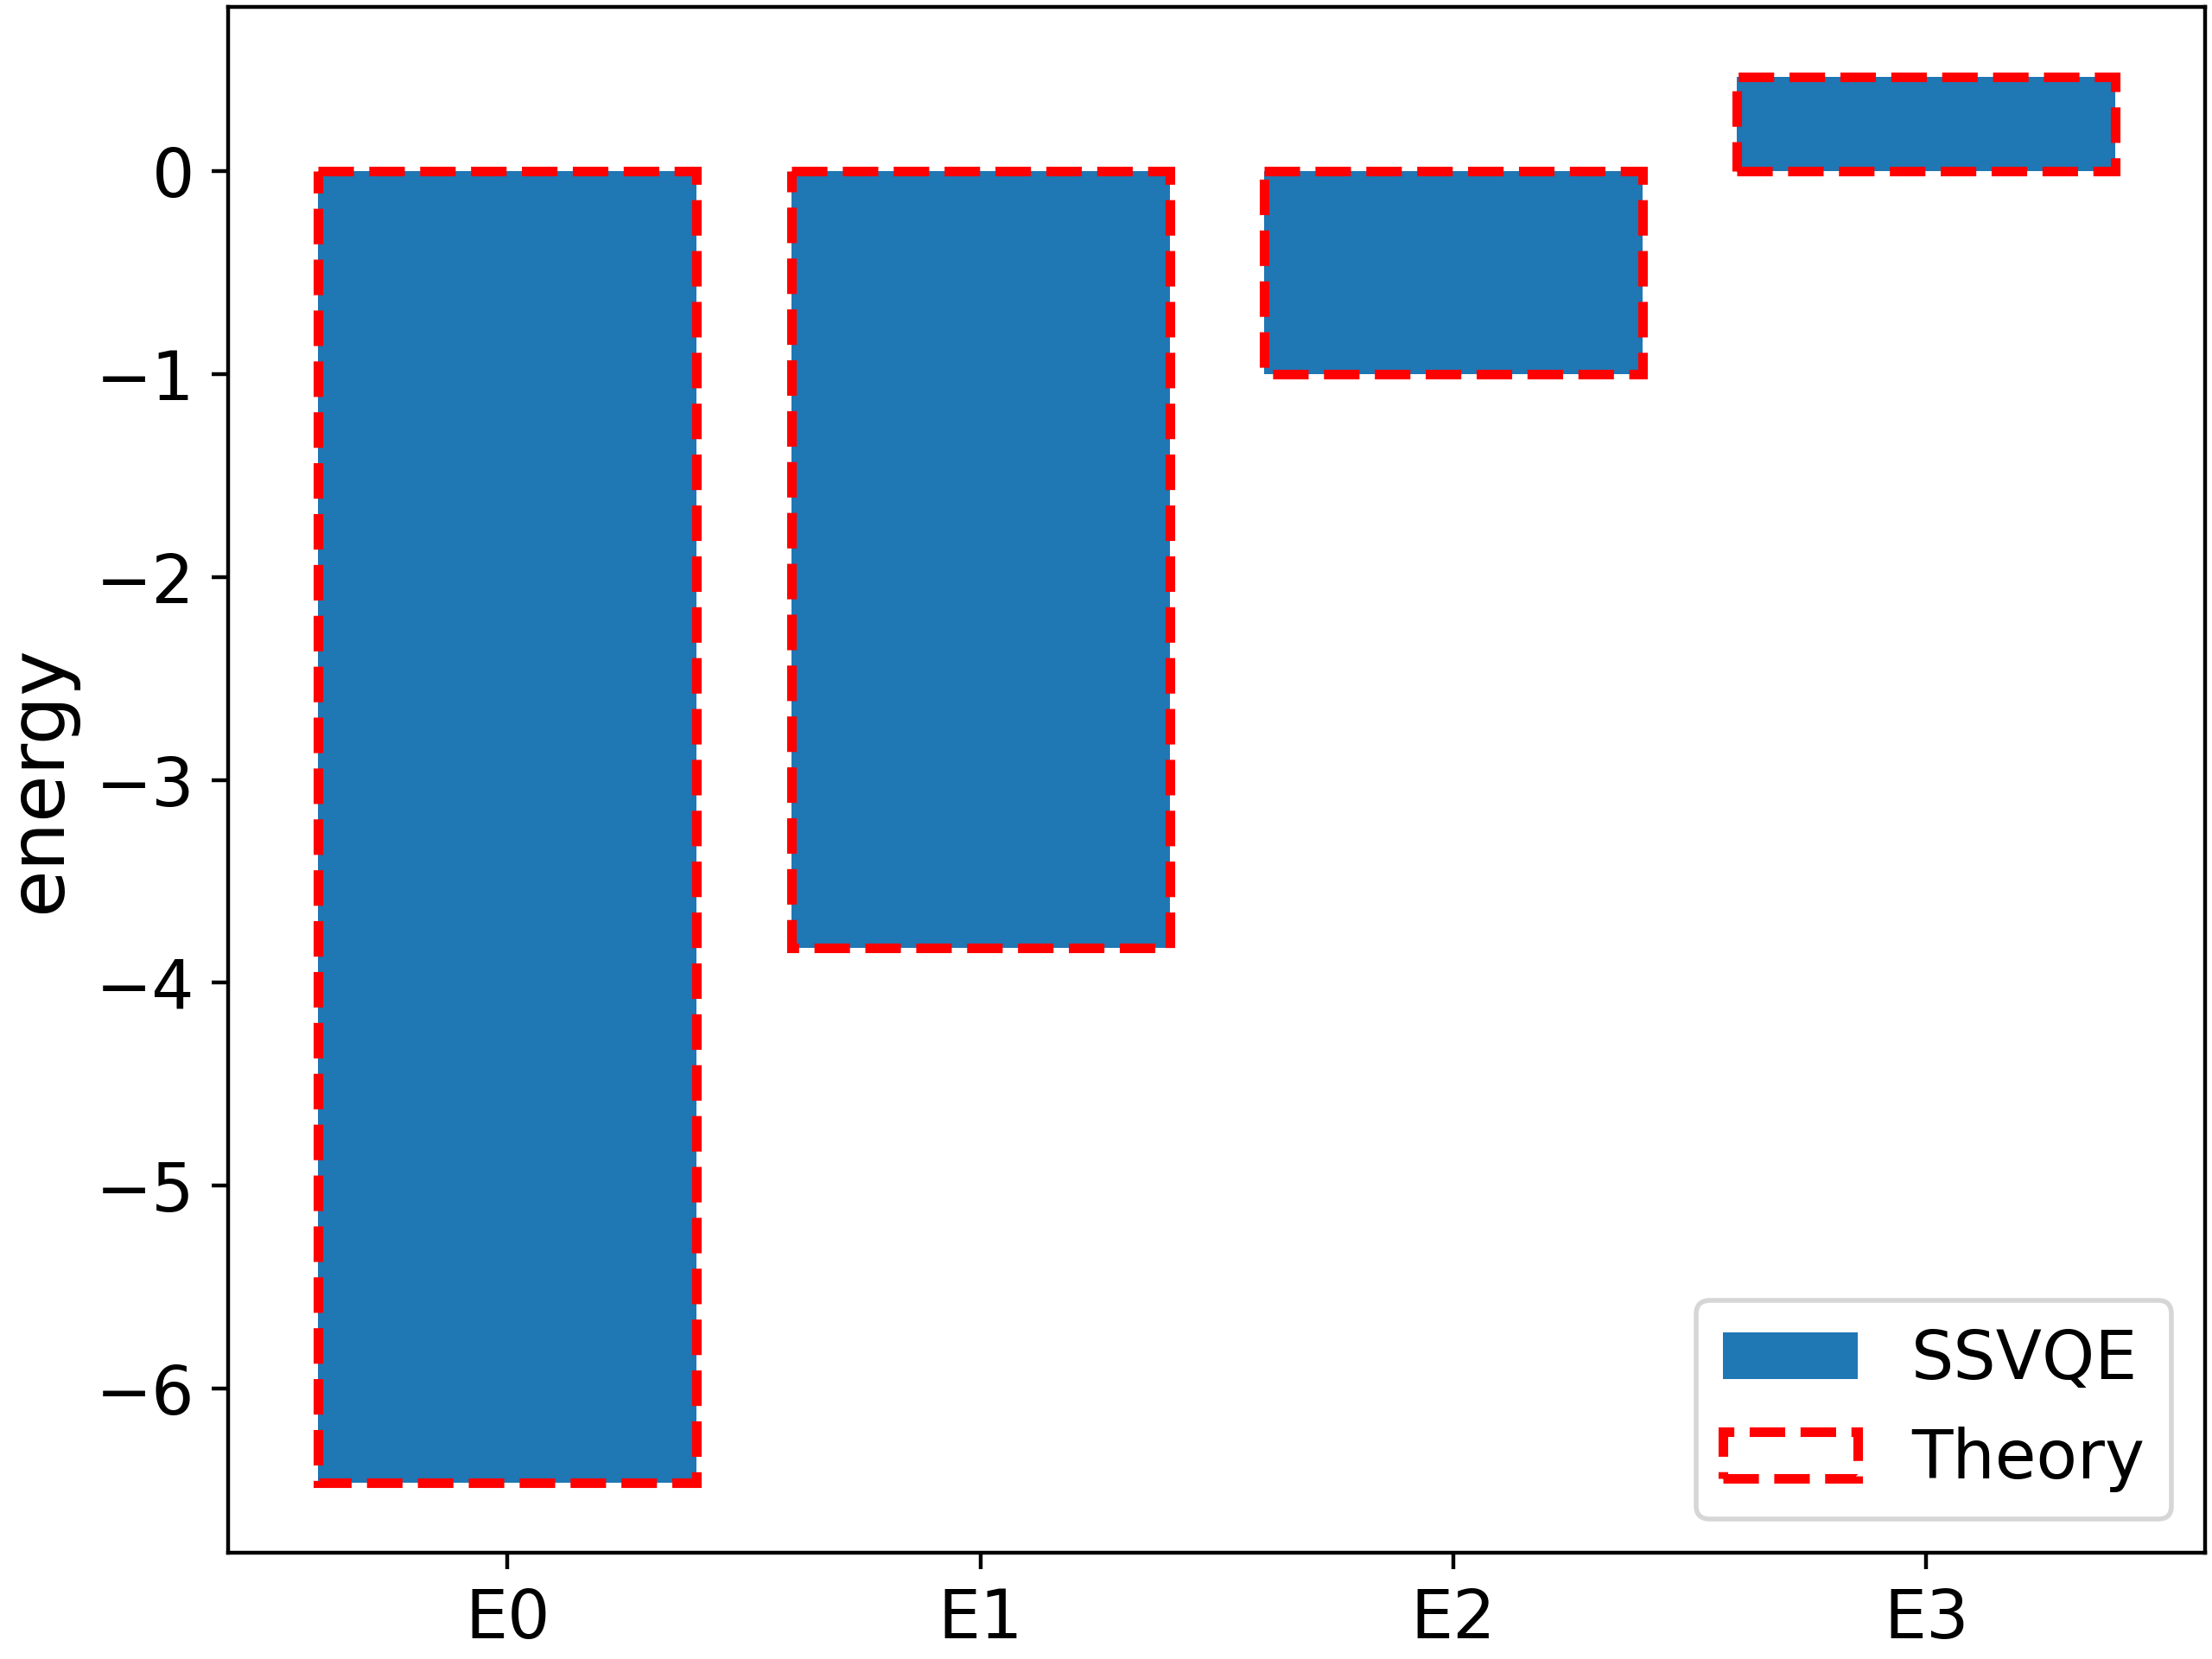
\includegraphics[width=1\linewidth]{5.4.2_figure/result.png}
	\caption{Simulation results of the SSVQE incorporating symmetries for 4-qubit Heisenberg Hamiltonian}
	\label{fig:SSVQE_result}
\end{figure}

This implementation completes training for the 4-qubit Heisenberg Hamiltonian in just seconds. One can take a look at the final results and generate a plot to compare the approximation results with the theoretical energies. In Fig.~\ref{{fig:SSVQE_result}, we show the simulation results for the four lowest state energies of the $4$-qubit Heisenberg Hamiltonian. Clearly, by incorporating inherent symmetries in SSVQE, it is possible to precisely approximate both ground and excited state energies in a resource-efficient manner.
